\documentclass[border=6pt,12pt]{standalone}
\usepackage{times}
\usepackage{amsmath,amssymb}
\usepackage{tikz}
\usetikzlibrary{arrows.meta, positioning, calc, fit, backgrounds}
\begin{document}
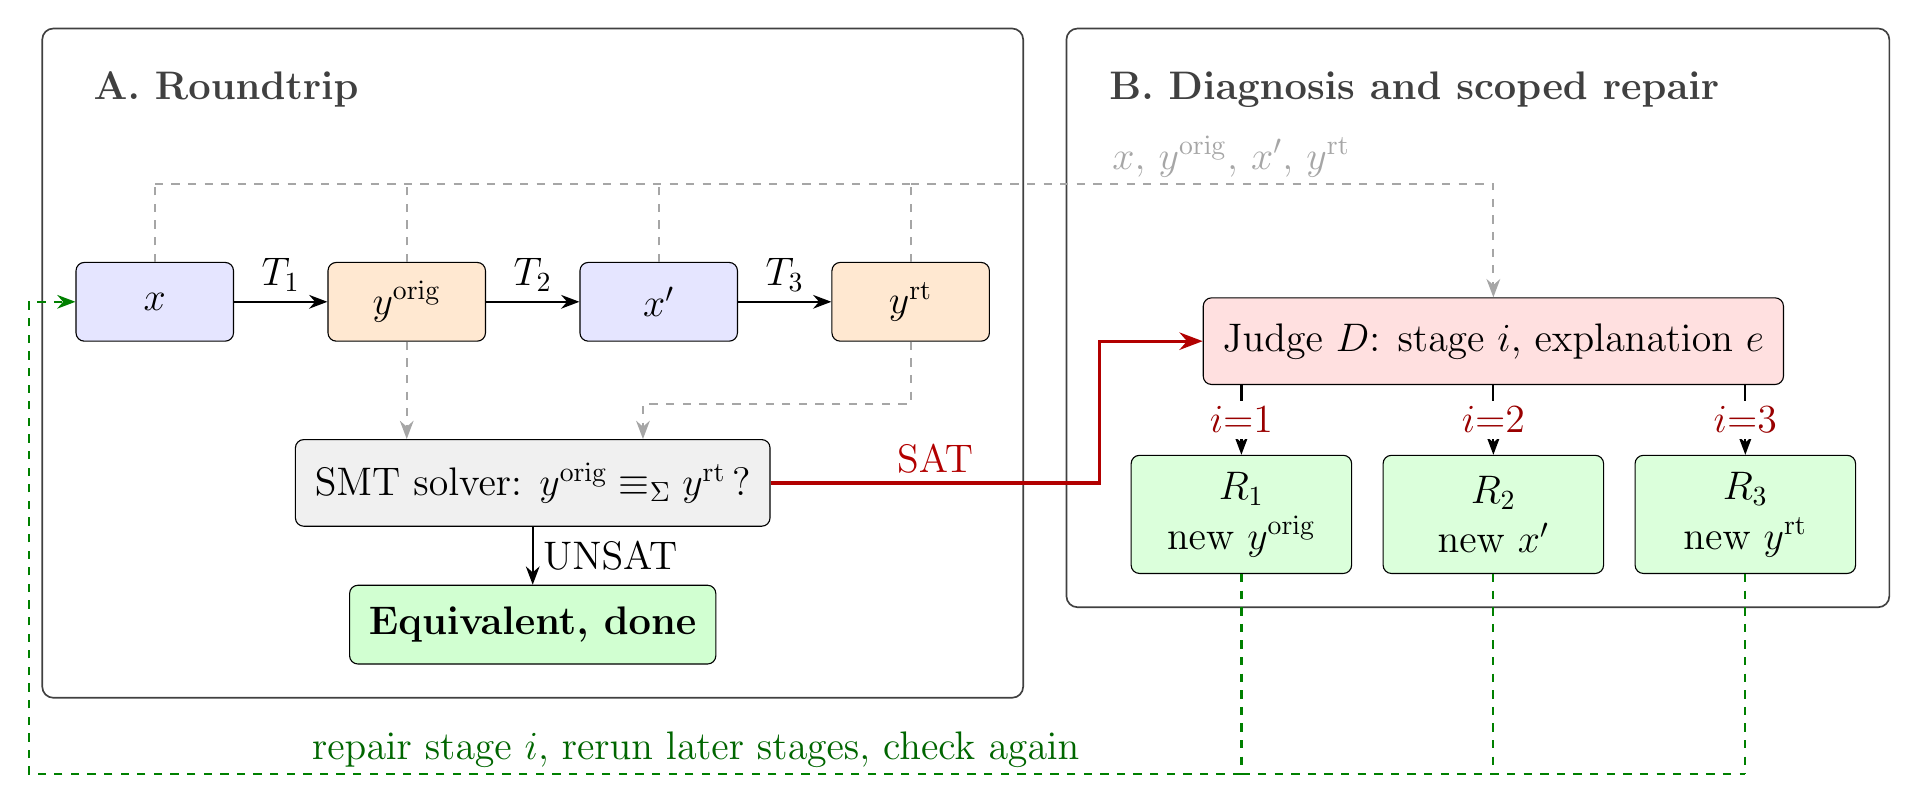
\begin{tikzpicture}[
    >=Stealth, font=\Large,
    nlbox/.style={draw, rounded corners=3pt, fill=blue!10, minimum width=2.0cm, minimum height=1.0cm, align=center},
    fmlbox/.style={draw, rounded corners=3pt, fill=orange!18, minimum width=2.0cm, minimum height=1.0cm, align=center},
    smtbox/.style={draw, rounded corners=3pt, fill=gray!12, minimum height=1.1cm, align=center, inner sep=7pt},
    succbox/.style={draw, rounded corners=3pt, fill=green!18, minimum height=1.0cm, align=center, inner sep=7pt, font=\Large\bfseries},
    diagbox/.style={draw, rounded corners=3pt, fill=red!12, minimum height=1.1cm, align=center, inner sep=7pt},
    repbox/.style={draw, rounded corners=3pt, fill=green!14, minimum width=2.8cm, minimum height=1.5cm, align=center, inner sep=5pt},
    paneltitle/.style={font=\Large\bfseries, text=black!75, anchor=west},
    panelframe/.style={draw=black!75, line width=0.6pt, rounded corners=4pt, inner sep=12pt},
    arrow/.style={->, thick, black},
    darrow/.style={->, thick, dashed, gray!70},
    satarrow/.style={->, very thick, red!70!black},
    reparrow/.style={->, thick, dashed, green!50!black},
    lbl/.style={fill=white, inner sep=2pt},
]
% ---- Panel A: roundtrip ----
\node[nlbox]  (x)     at (0,0)   {$x$};
\node[fmlbox] (yorig) at (3.2,0) {$y^{\mathrm{orig}}$};
\node[nlbox]  (xp)    at (6.4,0) {$x'$};
\node[fmlbox] (yrt)   at (9.6,0) {$y^{\mathrm{rt}}$};
\draw[arrow] (x)     -- node[above] {$T_1$} (yorig);
\draw[arrow] (yorig) -- node[above] {$T_2$} (xp);
\draw[arrow] (xp)    -- node[above] {$T_3$} (yrt);
\node[paneltitle] (titleA) at (-0.9, 2.7) {A.~Roundtrip};

\node[smtbox] (smt) at (4.8, -2.3) {SMT solver: $y^{\mathrm{orig}} \equiv_{\Sigma} y^{\mathrm{rt}}$\,?};
\draw[darrow] (yorig.south) -- (yorig.south |- smt.north);
\draw[darrow] (yrt.south) -- (9.6,-1.3) -- (6.2,-1.3) -- (6.2,0 |- smt.north);

\node[succbox] (success) at (4.8, -4.1) {Equivalent, done};
\draw[arrow] (smt) -- node[right] {UNSAT} (success);

% ---- Panel B: diagnosis and scoped repair ----
\node[diagbox] (D) at (17.0, -0.5) {Judge $D$: stage $i$, explanation $e$};
\node[paneltitle] (titleB) at (12.0, 2.7) {B.~Diagnosis and scoped repair};
\draw[satarrow] (smt.east) -- node[above] {SAT} (12.0, -2.3) |- (D.west);

\foreach \n in {x, yorig, xp, yrt} { \draw[darrow,-] (\n.north) -- (\n.north |- 0,1.5); }
\draw[darrow,-] (x.north |- 0,1.5) -- (yrt.north |- 0,1.5);
\draw[darrow] (yrt.north |- 0,1.5) -- node[lbl, above, pos=0.55] {$x,\,y^{\mathrm{orig}},\,x',\,y^{\mathrm{rt}}$} (17.0, 1.5) -- (D.north);

\node[repbox] (r1) at (13.8, -2.7) {$R_1$\\ new $y^{\mathrm{orig}}$};
\node[repbox] (r2) at (17.0, -2.7) {$R_2$\\ new $x'$};
\node[repbox] (r3) at (20.2, -2.7) {$R_3$\\ new $y^{\mathrm{rt}}$};
\draw[arrow] (D.south -| r1) -- node[lbl, pos=0.5, text=red!60!black] {$i{=}1$} (r1.north);
\draw[arrow] (D.south -| r2) -- node[lbl, pos=0.5, text=red!60!black] {$i{=}2$} (r2.north);
\draw[arrow] (D.south -| r3) -- node[lbl, pos=0.5, text=red!60!black] {$i{=}3$} (r3.north);

\foreach \r in {r1,r2,r3} { \draw[reparrow,-] (\r.south) -- (\r.south |- 0,-6.0); }
\draw[reparrow,-] (r1.south |- 0,-6.0) -- (r3.south |- 0,-6.0);
\draw[reparrow] (r1.south |- 0,-6.0) -- node[lbl, above, pos=0.45, text=green!40!black] {repair stage $i$, rerun later stages, check again} (-1.6,-6.0) -- (-1.6,0) -- (x.west);

\begin{scope}[on background layer]
  \node[panelframe, fit={(titleA) (x) (yrt) (smt) (success)}] {};
  \node[panelframe, fit={(titleB) (D) (r1) (r3)}] {};
\end{scope}
\end{tikzpicture}
\end{document}
